
%%%%%%%%%%%%%%%%%%%%%%%%%%%%%%%%%%%%%%%%%%%%%%%%%%%%%%%%%%%%%%%%%%%%%%%%%%%%%%%%
%Spenser Pulleyking
%Version: 0
%Description:
%Footnotes: 
%%%%%%%%%%%%%%%%%%%%%%%%%%%%%%%%%%%%%%%%%%%%%%%%%%%%%%%%%%%%%%%%%%%%%%%%%%%%%%%%
\pdfminorversion=4


%\documentclass[Conference]{IEEEtran}
\documentclass[letterpaper, 10 pt, conference]{ieeeconf}
\IEEEoverridecommandlockouts
% Some Computer Society conferences also require the compsoc mode option,
% but others use the standard conference format.
%
% If IEEEtran.cls has not been installed into the LaTeX system files,
% manually specify the path to it like:
% \documentclass[conference]{../sty/IEEEtran}



% Some very useful LaTeX packages include:
% (uncomment the ones you want to load)


% *** MISC UTILITY PACKAGES ***
%
%\usepackage{ifpdf}
% Heiko Oberdiek's ifpdf.sty is very useful if you need conditional
% compilation based on whether the output is pdf or dvi.
% usage:
% \ifpdf
%   % pdf code
% \else
%   % dvi code
% \fi
% The latest version of ifpdf.sty can be obtained from:
% http://www.ctan.org/pkg/ifpdf
% Also, note that IEEEtran.cls V1.7 and later provides a builtin
% \ifCLASSINFOpdf conditional that works the same way.
% When switching from latex to pdflatex and vice-versa, the compiler may
% have to be run twice to clear warning/error messages.



 



% *** CITATION PACKAGES ***
%
\usepackage{cite}
% cite.sty was written by Donald Arseneau
% V1.6 and later of IEEEtran pre-defines the format of the cite.sty package
% \cite{} output to follow that of the IEEE. Loading the cite package will
% result in citation numbers being automatically sorted and properly
% ``compressed/ranged". e.g., [1], [9], [2], [7], [5], [6] without using
% cite.sty will become [1], [2], [5]--[7], [9] using cite.sty. cite.sty's
% \cite will automatically add leading space, if needed. Use cite.sty's
% noadjust option (cite.sty V3.8 and later) if you want to turn this off
% such as if a citation ever needs to be enclosed in parenthesis.
% cite.sty is already installed on most LaTeX systems. Be sure and use
% version 5.0 (2009-03-20) and later if using hyperref.sty.
% The latest version can be obtained at:
% http://www.ctan.org/pkg/cite
% The documentation is contained in the cite.sty file itself.






% *** GRAPHICS RELATED PACKAGES ***
%
\ifCLASSINFOpdf
  \usepackage[pdftex]{graphicx}
  % declare the path(s) where your graphic files are
  \graphicspath{{./Figures/}{./figures}}
  % and their extensions so you won't have to specify these with
  % every instance of \includegraphics
  % \DeclareGraphicsExtensions{.pdf,.jpeg,.png}
\else
  % or other class option (dvipsone, dvipdf, if not using dvips). graphicx
  % will default to the driver specified in the system graphics.cfg if no
  % driver is specified.
  % \usepackage[dvips]{graphicx}
  % declare the path(s) where your graphic files are
  % \graphicspath{{../eps/}}
  % and their extensions so you won't have to specify these with
  % every instance of \includegraphics
  % \DeclareGraphicsExtensions{.eps}
\fi
% graphicx was written by David Carlisle and Sebastian Rahtz. It is
% required if you want graphics, photos, etc. graphicx.sty is already
% installed on most LaTeX systems. The latest version and documentation
% can be obtained at: 
% http://www.ctan.org/pkg/graphicx
% Another good source of documentation is "Using Imported Graphics in
% LaTeX2e" by Keith Reckdahl which can be found at:
% http://www.ctan.org/pkg/epslatex
%
% latex, and pdflatex in dvi mode, support graphics in encapsulated
% postscript (.eps) format. pdflatex in pdf mode supports graphics
% in .pdf, .jpeg, .png and .mps (metapost) formats. Users should ensure
% that all non-photo figures use a vector format (.eps, .pdf, .mps) and
% not a bitmapped formats (.jpeg, .png). The IEEE frowns on bitmapped formats
% which can result in "jaggedy"/blurry rendering of lines and letters as
% well as large increases in file sizes.
%
% You can find documentation about the pdfTeX application at:
% http://www.tug.org/applications/pdftex





% *** MATH PACKAGES ***
%
\usepackage{amsmath}
% A popular package from the American Mathematical Society that provides
% many useful and powerful commands for dealing with mathematics.
%
% Note that the amsmath package sets \interdisplaylinepenalty to 10000
% thus preventing page breaks from occurring within multiline equations. Use:
%\interdisplaylinepenalty=2500
% after loading amsmath to restore such page breaks as IEEEtran.cls normally
% does. amsmath.sty is already installed on most LaTeX systems. The latest
% version and documentation can be obtained at:
% http://www.ctan.org/pkg/amsmath


\usepackage{amssymb}  % assumes amsmath package installed

\usepackage{times}

% *** SPECIALIZED LIST PACKAGES ***
%
%\usepackage{algorithmic}
% algorithmic.sty was written by Peter Williams and Rogerio Brito.
% This package provides an algorithmic environment fo describing algorithms.
% You can use the algorithmic environment in-text or within a figure
% environment to provide for a floating algorithm. Do NOT use the algorithm
% floating environment provided by algorithm.sty (by the same authors) or
% algorithm2e.sty (by Christophe Fiorio) as the IEEE does not use dedicated
% algorithm float types and packages that provide these will not provide
% correct IEEE style captions. The latest version and documentation of
% algorithmic.sty can be obtained at:
% http://www.ctan.org/pkg/algorithms
% Also of interest may be the (relatively newer and more customizable)
% algorithmicx.sty package by Szasz Janos:
% http://www.ctan.org/pkg/algorithmicx




% *** ALIGNMENT PACKAGES ***
%
%\usepackage{array}
% Frank Mittelbach's and David Carlisle's array.sty patches and improves
% the standard LaTeX2e array and tabular environments to provide better
% appearance and additional user controls. As the default LaTeX2e table
% generation code is lacking to the point of almost being broken with
% respect to the quality of the end results, all users are strongly
% advised to use an enhanced (at the very least that provided by array.sty)
% set of table tools. array.sty is already installed on most systems. The
% latest version and documentation can be obtained at:
% http://www.ctan.org/pkg/array


% IEEEtran contains the IEEEeqnarray family of commands that can be used to
% generate multiline equations as well as matrices, tables, etc., of high
% quality.




% *** SUBFIGURE PACKAGES ***
%\ifCLASSOPTIONcompsoc
%  \usepackage[caption=false,font=normalsize,labelfont=sf,textfont=sf]{subfig}
%\else
%  \usepackage[caption=false,font=footnotesize]{subfig}
%\fi
% subfig.sty, written by Steven Douglas Cochran, is the modern replacement
% for subfigure.sty, the latter of which is no longer maintained and is
% incompatible with some LaTeX packages including fixltx2e. However,
% subfig.sty requires and automatically loads Axel Sommerfeldt's caption.sty
% which will override IEEEtran.cls' handling of captions and this will result
% in non-IEEE style figure/table captions. To prevent this problem, be sure
% and invoke subfig.sty's "caption=false" package option (available since
% subfig.sty version 1.3, 2005/06/28) as this is will preserve IEEEtran.cls
% handling of captions.
% Note that the Computer Society format requires a larger sans serif font
% than the serif footnote size font used in traditional IEEE formatting
% and thus the need to invoke different subfig.sty package options depending
% on whether compsoc mode has been enabled.
%
% The latest version and documentation of subfig.sty can be obtained at:
% http://www.ctan.org/pkg/subfig




% *** FLOAT PACKAGES ***
%
%\usepackage{fixltx2e}
% fixltx2e, the successor to the earlier fix2col.sty, was written by
% Frank Mittelbach and David Carlisle. This package corrects a few problems
% in the LaTeX2e kernel, the most notable of which is that in current
% LaTeX2e releases, the ordering of single and double column floats is not
% guaranteed to be preserved. Thus, an unpatched LaTeX2e can allow a
% single column figure to be placed prior to an earlier double column
% figure.
% Be aware that LaTeX2e kernels dated 2015 and later have fixltx2e.sty's
% corrections already built into the system in which case a warning will
% be issued if an attempt is made to load fixltx2e.sty as it is no longer
% needed.
% The latest version and documentation can be found at:
% http://www.ctan.org/pkg/fixltx2e


%\usepackage{stfloats}
% stfloats.sty was written by Sigitas Tolusis. This package gives LaTeX2e
% the ability to do double column floats at the bottom of the page as well
% as the top. (e.g., "\begin{figure*}[!b]" is not normally possible in
% LaTeX2e). It also provides a command:
%\fnbelowfloat
% to enable the placement of footnotes below bottom floats (the standard
% LaTeX2e kernel puts them above bottom floats). This is an invasive package
% which rewrites many portions of the LaTeX2e float routines. It may not work
% with other packages that modify the LaTeX2e float routines. The latest
% version and documentation can be obtained at:
% http://www.ctan.org/pkg/stfloats
% Do not use the stfloats baselinefloat ability as the IEEE does not allow
% \baselineskip to stretch. Authors submitting work to the IEEE should note
% that the IEEE rarely uses double column equations and that authors should try
% to avoid such use. Do not be tempted to use the cuted.sty or midfloat.sty
% packages (also by Sigitas Tolusis) as the IEEE does not format its papers in
% such ways.
% Do not attempt to use stfloats with fixltx2e as they are incompatible.
% Instead, use Morten Hogholm'a dblfloatfix which combines the features
% of both fixltx2e and stfloats:
%
% \usepackage{dblfloatfix}
% The latest version can be found at:
% http://www.ctan.org/pkg/dblfloatfix




% *** PDF, URL AND HYPERLINK PACKAGES ***
%
%\usepackage{url}
% url.sty was written by Donald Arseneau. It provides better support for
% handling and breaking URLs. url.sty is already installed on most LaTeX
% systems. The latest version and documentation can be obtained at:
% http://www.ctan.org/pkg/url
% Basically, \url{my_url_here}.




% *** Do not adjust lengths that control margins, column widths, etc. ***
% *** Do not use packages that alter fonts (such as pslatex).         ***
% There should be no need to do such things with IEEEtran.cls V1.6 and later.
% (Unless specifically asked to do so by the journal or conference you plan
% to submit to, of course. )


% correct bad hyphenation here
\hyphenation{op-tical net-works semi-conduc-tor}
\pagenumbering{gobble}

\begin{document}
%
% paper title
% Titles are generally capitalized except for words such as a, an, and, as,
% at, but, by, for, in, nor, of, on, or, the, to and up, which are usually
% not capitalized unless they are the first or last word of the title.
% Linebreaks \\ can be used within to get better formatting as desired.
% Do not put math or special symbols in the title.
\title{Flexure Hinge-based Biomimetic Thumb with a Rolling-Surface Metacarpal Joint}


% author names and affiliations
% use a multiple column layout for up to three different
% affiliations
\author{Spenser Pulleyking, Joshua Schultz, \textit{Senior Member, IEEE}}

\thanks{All authors are with the Department of Mechanical Engineering, the University of Tulsa, Tulsa, OK 74104, USA. Research supported by NSF NRI 1427250. Thanks to Albert Okoh, Dipayan Das and Braeden Williams for their dedicated work on manufacturing small robotic parts for this research.}


% conference papers do not typically use \thanks and this command
% is locked out in conference mode. If really needed, such as for
% the acknowledgment of grants, issue a \IEEEoverridecommandlockouts
% after \documentclass

% for over three affiliations, or if they all won't fit within the width
% of the page, use this alternative format:
% 
%\author{\IEEEauthorblockN{Michael Shell\IEEEauthorrefmark{1},
%Homer Simpson\IEEEauthorrefmark{2},
%James Kirk\IEEEauthorrefmark{3}, 
%Montgomery Scott\IEEEauthorrefmark{3} and
%Eldon Tyrell\IEEEauthorrefmark{4}}
%\IEEEauthorblockA{\IEEEauthorrefmark{1}School of Electrical and Computer Engineering\\
%Georgia Institute of Technology,
%Atlanta, Georgia 30332--0250\\ Email: see http://www.michaelshell.org/contact.html}
%\IEEEauthorblockA{\IEEEauthorrefmark{2}Twentieth Century Fox, Springfield, USA\\
%Email: homer@thesimpsons.com}
%\IEEEauthorblockA{\IEEEauthorrefmark{3}Starfleet Academy, San Francisco, California 96678-2391\\
%Telephone: (800) 555--1212, Fax: (888) 555--1212}
%\IEEEauthorblockA{\IEEEauthorrefmark{4}Tyrell Inc., 123 Replicant Street, Los Angeles, California 90210--4321}}



% use for special paper notices
%\IEEEspecialpapernotice{(Invited Paper)}




% make the title area
\maketitle

% As a general rule, do not put math, special symbols or citations
% in the abstract
\begin{abstract}
The human thumb's state contribution to grasping and dexterous manipulation of objects is a function of the kinematic multiplicity of joints and structure of the bones, joints, and ligaments. This paper looks at the design and evaluation of a human-like thumb for use in a robotic hand, where the thumb's state contribution to grasping and dexterous manipulation is a function of a simplified kinematic model based on that of the human thumb, but also on empirical trials of surgical techniques to retain functionality while reducing the number of joints in the thumb. Motion Capture Data of the End Effector is analyzed with the measured excursion of the tendons to determine the relationship between tendon velocities and task-space velocities. After validating the procedure experimentally, a simplified metric is proposed to represent this data, and shows that our prototype is predicted to have a relatively smooth mapping between tendon excursion velocity and end effector velocity. 
\end{abstract}

% no keywords




% For peer review papers, you can put extra information on the cover
% page as needed:
% \ifCLASSOPTIONpeerreview
% \begin{center} \bfseries EDICS Category: 3-BBND \end{center}
% \fi
%
% For peerreview papers, this IEEEtran command inserts a page break and
% creates the second title. It will be ignored for other modes.
\IEEEpeerreviewmaketitle

\section{Introduction}
% no \IEEEPARstart

The human hand occupies a unique niche among biomechanics and industrial robotic manipulators alike: although there is no agreed upon optimal kinematic model for the human hand, it enables versatility and dexterity among many different tasks \cite{vfingers} \cite{ss}. Robotic hand research has generated a vast and diverse set of kinematic models, even when modeling the human thumb itself. For instance, at least four modes of description of the Carpometacarpal Joint (CMC) emerge when attempting to extract kinematic modalities from Monte Carlo simulations of biological data \cite{santos2006reported} \cite{niehues} \cite{nana}. Learning from past robotic hands' limitations, we seek to reduce the complexity of the design space by minimizing the degrees of freedom required to functionally contribute to grasping objects. As an indicator of real-world grasp quality, we take empirically validated joint angle parameters for Arthrodesis, a surgical fixation of the Metacarpal-Phalangeal Joint (MCP) that preserves the functionality of the hand, and develop a robotic thumb based on these parameters, to retain both the overall hand functionality and the desired joint minimization.

The CMC is often considered the most difficult to model \cite{santos2006reported}. The next joint, the MCP, experiences relatively little angular motion in many daily motions \cite{steiger}, which along with surgical data on the process of Arthrodesis suggests that the MCP can be fixed in place without great loss of grasping functionality throughout the hand \cite{biorob}. Finally, the Distal Phalangeal joint (DP) is the simplest to model, and our design does not deviate much from other robotic hands in treating it as a pin joint \cite{iCub} \cite{pisahand}.


%Figure: Photo of the thumb
\begin{figure}
	\centering
	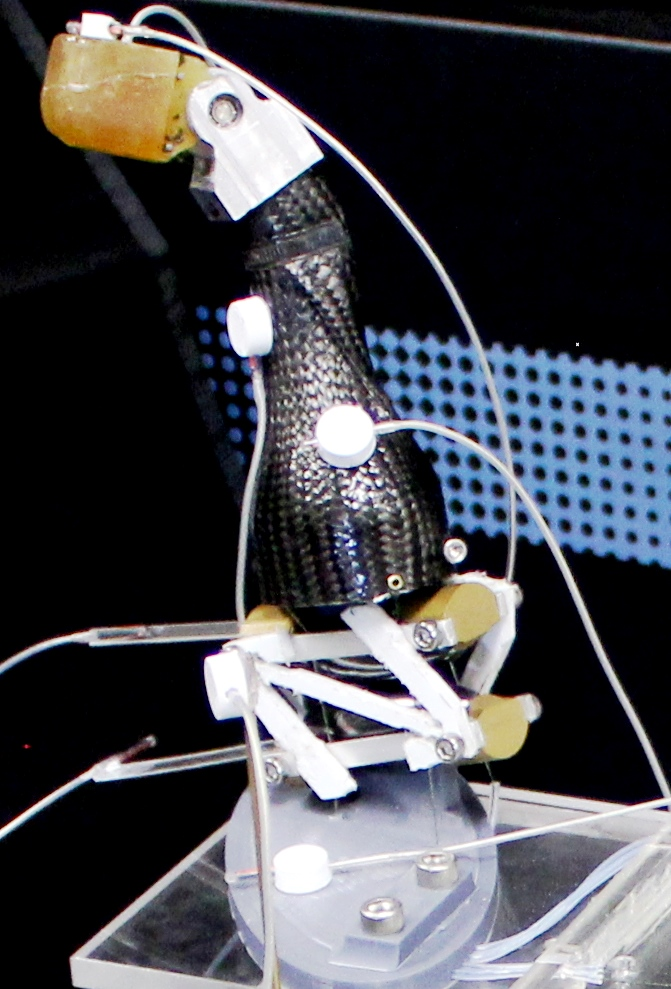
\includegraphics[width = .5\columnwidth]{Figures/f1.jpg}
	\caption{Photograph of the prototype model with mounted magnetic field distortion-based motion/position sensors. Their response to thumb movement is captured on a Polhemus Liberty\texttrademark \medspace unit, partially shown in the background. }\label{thumbphoto}
	\vspace{-15pt}
\end{figure}



Orthopaedic surgery has found that, while severe arthritis is distributed across different joints for different people, that the fusion or ``fixing" of certain hand joints more effectively improves post-surgery outcomes than other hand joints, as measured by ease and comfort of motion. One of well-established parametric sets for human thumb Arthrodesis, the surgical procedure of fixing a joint, is the Steiger Arthrodesis, which dictates the fixation angles \cite{steiger}. We realize both bones in a single part geometry, whose outer surface represents the metacarpal and proximal phalanx as one static surface. The surface geometry was defined to approximate the contours of the thenar region of the palm, as it merges with the palm. 

To summarize these simplifications: the Carpometacarpal Joint action is represented by a rolling ellipsoidal joint, and the Metacarpal-Phalangeal Joint is represented by a fixed joint based on surgical Arthrodesis parameters. Alternatively, the Distal Phalangeal Joint remains similar to most other robotic thumbs---it is treated as a pin joint at the interface between the Middle Phalanx and Distal Phalanx. We also seek in this paper to demonstrate a mechanical replacement for the CMC using magnetic ceramic rolling-surfaces and flexure hinges. In our prior work, an earlier prototype's workspace volume after an Arthrodesis of the MCP joint was calculated and compared to previous prototypes and that of a human thumb \cite{biorob}. Thus, our problem statement is to determine how to employ the usage of flexure hinges to properly constrain the CMC, and to verify the accuracy of this constraint by calculating the tendon excursions and their relative velocities. These values are presented as a weighted point cloud in Figure 7. 


\section{Bi-Ellipsoidal Rigid Body Model of the CMC Joint}
The proposed CMC joint is a nontraditional compliant joint, thus we seek to determine its applicability as a model of the CMC's functionality. Our previous work has shown that this choice of CMC modeling does not significantly reduce the volume of the end effector's workspace \cite{biorob}. Also, state of the art robotic hands like the \textit{Shadowhand} and \textit{iCub Robotic Hand} approximate the CMC as two orthogonal pin joints with some offset between them, and the \textit{Shadowhand} requires a third degree of freedom to function, rotation about the base of the thumb, to approximate the biological motion of ``supination". Even though there is no biological analog to the \textit{Shadowhand} where supination motion is generated via a third degree of freedom, this added complexity is vital to the functionality of the overall device, as grasp calibration testing alongside a human hand with a data-glove has shown that controlling thumb tip orientation relative to that of the fingers is critical to most grasps \cite{kingcakebaby}. Since three pin joints replicating two rolling-surface joints is somewhat redundant, our design explores the possibility of a system coupling that results in a fully constrained joint with 2 fundamental degrees of freedom to match the biological behaviour. Another key reason for choosing these ceramic ellipsoids was their magnetism, shown in Figure 3: the orientation generates a field equilibrium that resists displacement, thus practically mimicking the behaviour of soft cartilage in the fingers when unloaded. This magnetism is necessary in terms of flexure/extension to prevent any rolling without slipping; as the magnetic fields are kept in opposition and symmetric throughout the range of motion, the magnetism will always act as a restoring force to a mean point of extension of all tendons. 

Our bi-ellipsoidal CMC design can be summarized as follows: two identical (at least up to manufacturing variations)
 ellipses are constrained to be in rolling-without-slipping contact when cross-linked through their foci; these ellipses represent 2D cross sections of a 3D analogous system that introduces an orthogonal degree of freedom by also allowing for rotation of the upper ellipsoid about it's major prolate axis. The significance of this design is that the difference in magnitude between their major and minor axes is what makes them prolate, and allows us to design for arbitrary external forces while still making a distinction between Abduction/Adduction motion and Flexion/Extension motion. If their major and minor radial magnitudes were equivalent, both would be spheres, and tendon placement relative to the axes would not be able to influence the stability of grasping as parameterized by the two orthogonal degrees of freedom in the joint. This relationship has been well known in mechanical theory for over a century when applied to ellipses in 2D, but has never before been applied to ellipsoids in 3D, which necessitates the development of constraining ligament analogs, the flexure hinges. This extension to 3D is crucial to the thumb model, as the thumb's CMC is NOT planar, meaning mechanical design is needed to allow the thumb to rotate about an additional axis. The ``ligament analogs" follow from this, as shown in Table 1. If the thumb were planar, 2D ellipses instead of 3D ellipsoids would require pins through the foci. The result of this is thus inversion of the biological surfaces' Gaussian curvature from negative to positive: these surfaces of the CMC, which are hyperboloidal surface patches, become rolling-without-slipping ellipsoidal surface patches, which are easily mapped as moderate deformations of a ruled surface. These ruled surfaces thus allow for fast modeling and incorporation into the generalized coordinates of the system. The ellipsoids' major prolate axes are constrained to always be in the same plane by the mechanism described in this paper. Thus, only two motions are possible: the upper ellipsoid rolls about a minor circumference of the lower ellipse, or about the major ellipsoidal cross-section of the lower ellipse. The action is best understood by watching the video of the prototype's motion presented with this paper.

\begin{table}
\vspace{4pt}
	\centering
	\caption{Functional Reduction of Joint Space for Biomimetic Thumb}\label{DOFchoice}
	\begin{tabular}{c|c|c}
		Natural Analog & Dexterous Function & Replaced By \\
		\hline
		Trapezium Bone & CMC Base & Lower Ceramic Ellipsoid \\
		Trapezoid Bone & CMC Base & Lower Ceramic Ellipsoid \\
		Radial Ligament& Abd. Constraint & Volar Flexure Hinge\\
		Ulnar Ligament & Abd. Constraint & Dorsal Flexure Hinge\\
		Metacarpal & CMC Linkage & Upper Ceramic Ellipsoid\\
		Proximal Phlx. & Joint-Linkage & (Fixed)/Carbon Fiber Hull\\
	    Distal Phlx. & End Effector Joint & Pin Joint\\
		\hline
	\end{tabular}
\end{table}

\section{Flexure Hinges as ligaments and constraints of the CMC Joint}
Two flexure hinges are required, one dorsal and one volar, to replicate the constraining action of the natural CMC ligaments. The dorsal and volar  flexure hinges' main purpose is to provide a rigid linkage between the foci of the upper and lower ellipsoids, as shown in Figure 3. This mechanism prevents certain movements from occurring: slippage between the ellipsoids, subluxation, separation, and spinning about the contact point. Considering the planar case of ellipses, these constraints are equivalent to those of a traditional four-bar mechanism, where one of the linkages is defined by a point of continuous contact. This constraint keeps the two ellipsoids in contact at all times (a condition which is supported by the magnetic attraction of the ceramics) so that they roll on one another without slipping when the thumb is moving or applying force to an external object. The central advantage of using flexure hinges is that they are able to accommodate any misalignment that could occur, while any misalignment in a similarly scaled hinge would likely cause it to bind.

As seen in Figure 6, the flexure hinges' geometry is designed in such a way that they are their own mechanical stops, as machined. The range of motion of the flexure hinges is half that of the overall abduction/adduction range of motion, listed in Table 1. Initially, our results with double c-type flexure hinges have been promising: after approximately 1200 cycles of full range of motion cycles, neither of the flexure hinges have had to be replaced. 

The use of flexure hinges in biomimetic robotics is not well known, although there have been efforts to explore this design space \cite{havd}. The geometry of flexure hinges is an active area of research, as many other geometries are possible besides c-type hinges \cite{yodel}. While magnetism is not present in biological joints as a returning force, it is somewhat analogous to a gentle returning force caused by the expansion of cartilage and other tissues when we are at rest \cite{santos2006reported}.

Both the mechanical constraints imposed by the flexure hinges and the magnetic stabilization imposed by the ceramics work together to keep the joint aligned. A complete force-torque analysis of the device is planned, once the device is installed into the TU Hand's compliant actuation: when caging an object, a grasp's stability is directly limited by the weakest force vector in the flexion direction (into the grasped object), so the external forcing capabilities of the thumb is determined simultaneously with the other opposing digits, due to the compliance inherent to the system. As tendon-driven actuation in robotic hands has historically been bulky and difficult to incorporate into a lightweight design, the TU hand is designed to utilize an established compliant mechanism \cite{homies}.

The flexure hinges are manufactured to exact tolerances required to maintain a consistent degree of axial tension about the most narrow cross-section of the hinge, based on the model of the ellipsoidal geometry. However, the ceramic magnetic ellipsoids are very low cost, and thus have poor tolerances when implemented as ellipsoids; they are roughly blended with a rectangular prism similar to the ideal ellipsoid. Thus, we designed the flexure hinges to be relaxed when in the resting position, and slightly tensile when fully extended into abduction or adduction at any degree of flexion/extension. The effect of this is that for anywhere in the workspace, the flexure hinges fully constrain the point of contact between the ellipsoids to follow a one-to-one path; that is, it's gradient can be computed.

%Figure: Photo of the thumb
\begin{figure}
	\vspace{7pt}
	\centering
	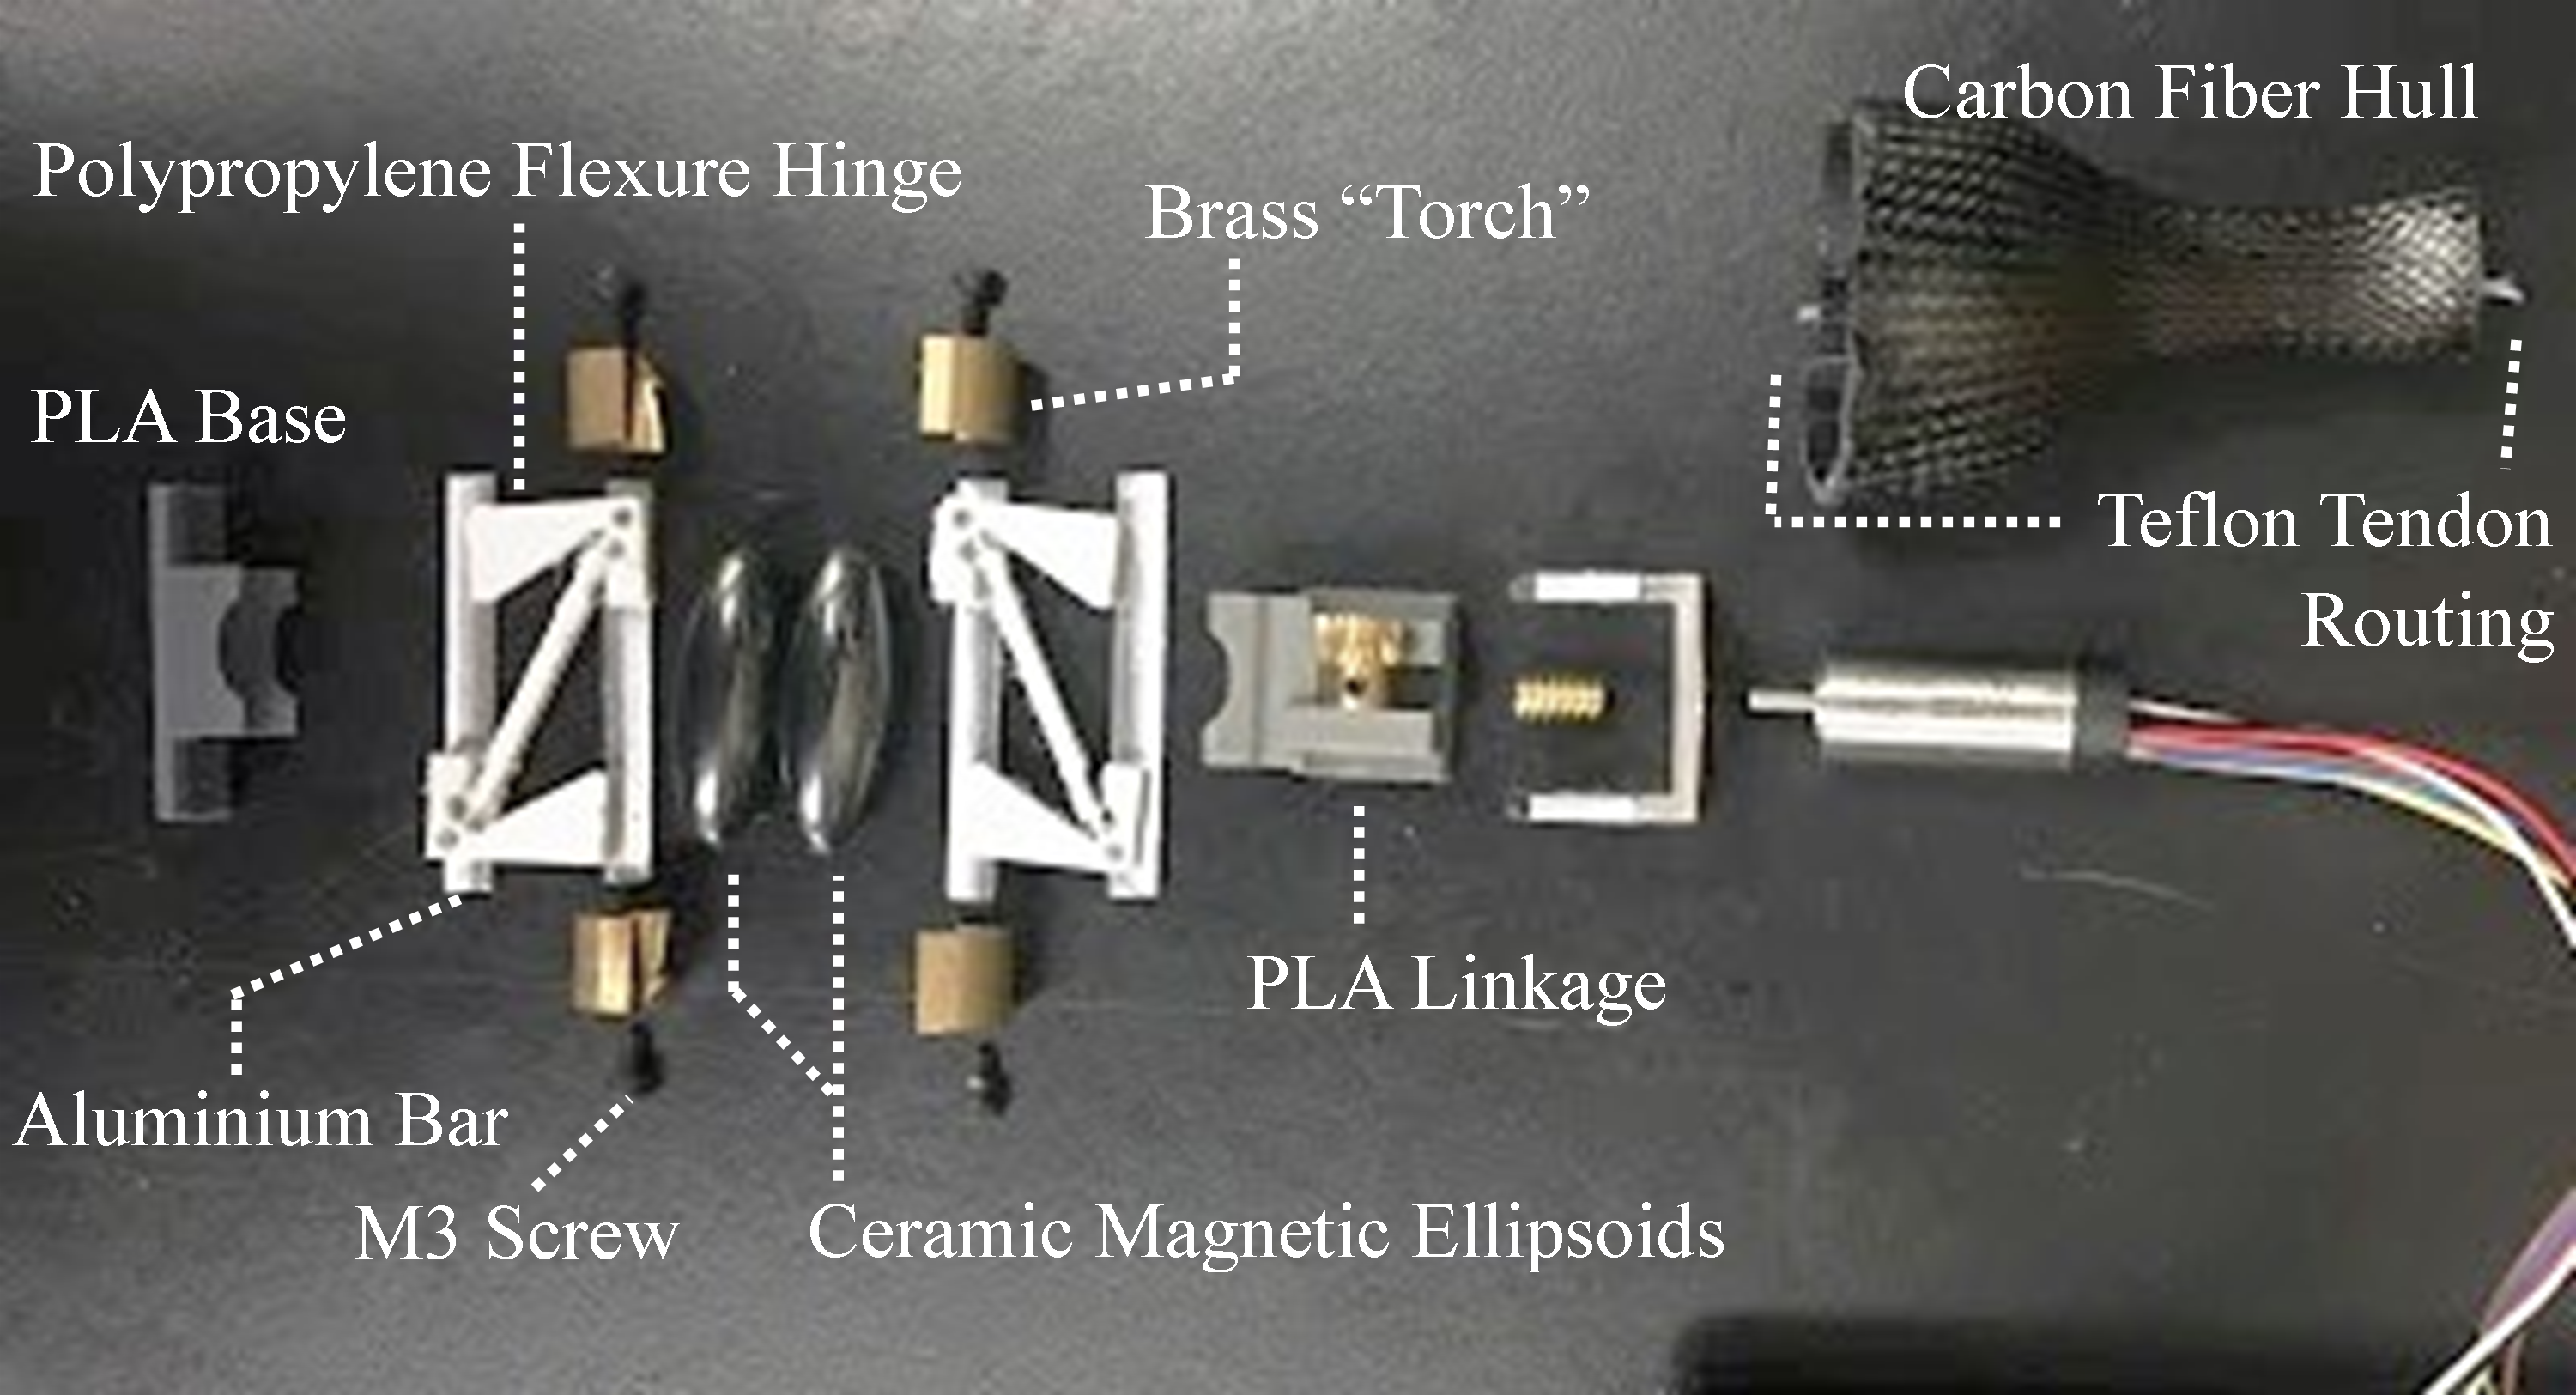
\includegraphics[width = 1\columnwidth]{Figures/A4.png}
	\caption{Photograph of the prototype model in exploded view. This prototype is based on the proposed Steiger Arthrodesis at the metacarpal (MP) joint of the thumb, and also on a novel carpometacarpal (CMC) ellipsoidal joint. The locations of the interphalangeal (IP) joint and the ellipsoids of the CMC joint are rigid, but slippage at the CMC allows compliant control. Four brass ``torches" are machined to enclose the rotation of the prolate ellipsoid ends, and dorsal and volar flexure hinges are machined similarly, although one is rotated so they act in continuous opposition. To allow for under-actuated grasping, the motion of the IP joint is mechanically coupled with that of the CMC joint. Brass Torches are manufactured to secure the flexure hinges in place, and connected via aluminum bars (seen beneath the flexure hinges). }\label{thumbphoto}
	\vspace{-15pt}
\end{figure}

%Figure: Photo of the thumb
\begin{figure}
	\centering
    \vspace{7pt}
	\includegraphics[width = .7\columnwidth]{Figures/B.png}
	\caption{Photograph of the prototype CMC model's scalar magnetic field superimposed over a model of the upper and lower ellipsoids. The field acts normal to the minor axis of the ellipsoids. This creates a unique opportunity to take advantage of cross-linking between the foci (action is along the white solid lines which terminate at the foci) to stabilize the entire CMC joint and prevent any slippage between the ceramic elements, much like how our connective tissues keep our bones moving, as if in rolling contact at the ends.}\label{thumbphoto}
	\vspace{-15pt}
\end{figure}


\begin{figure}
    \vspace{6pt}
	\centering
    {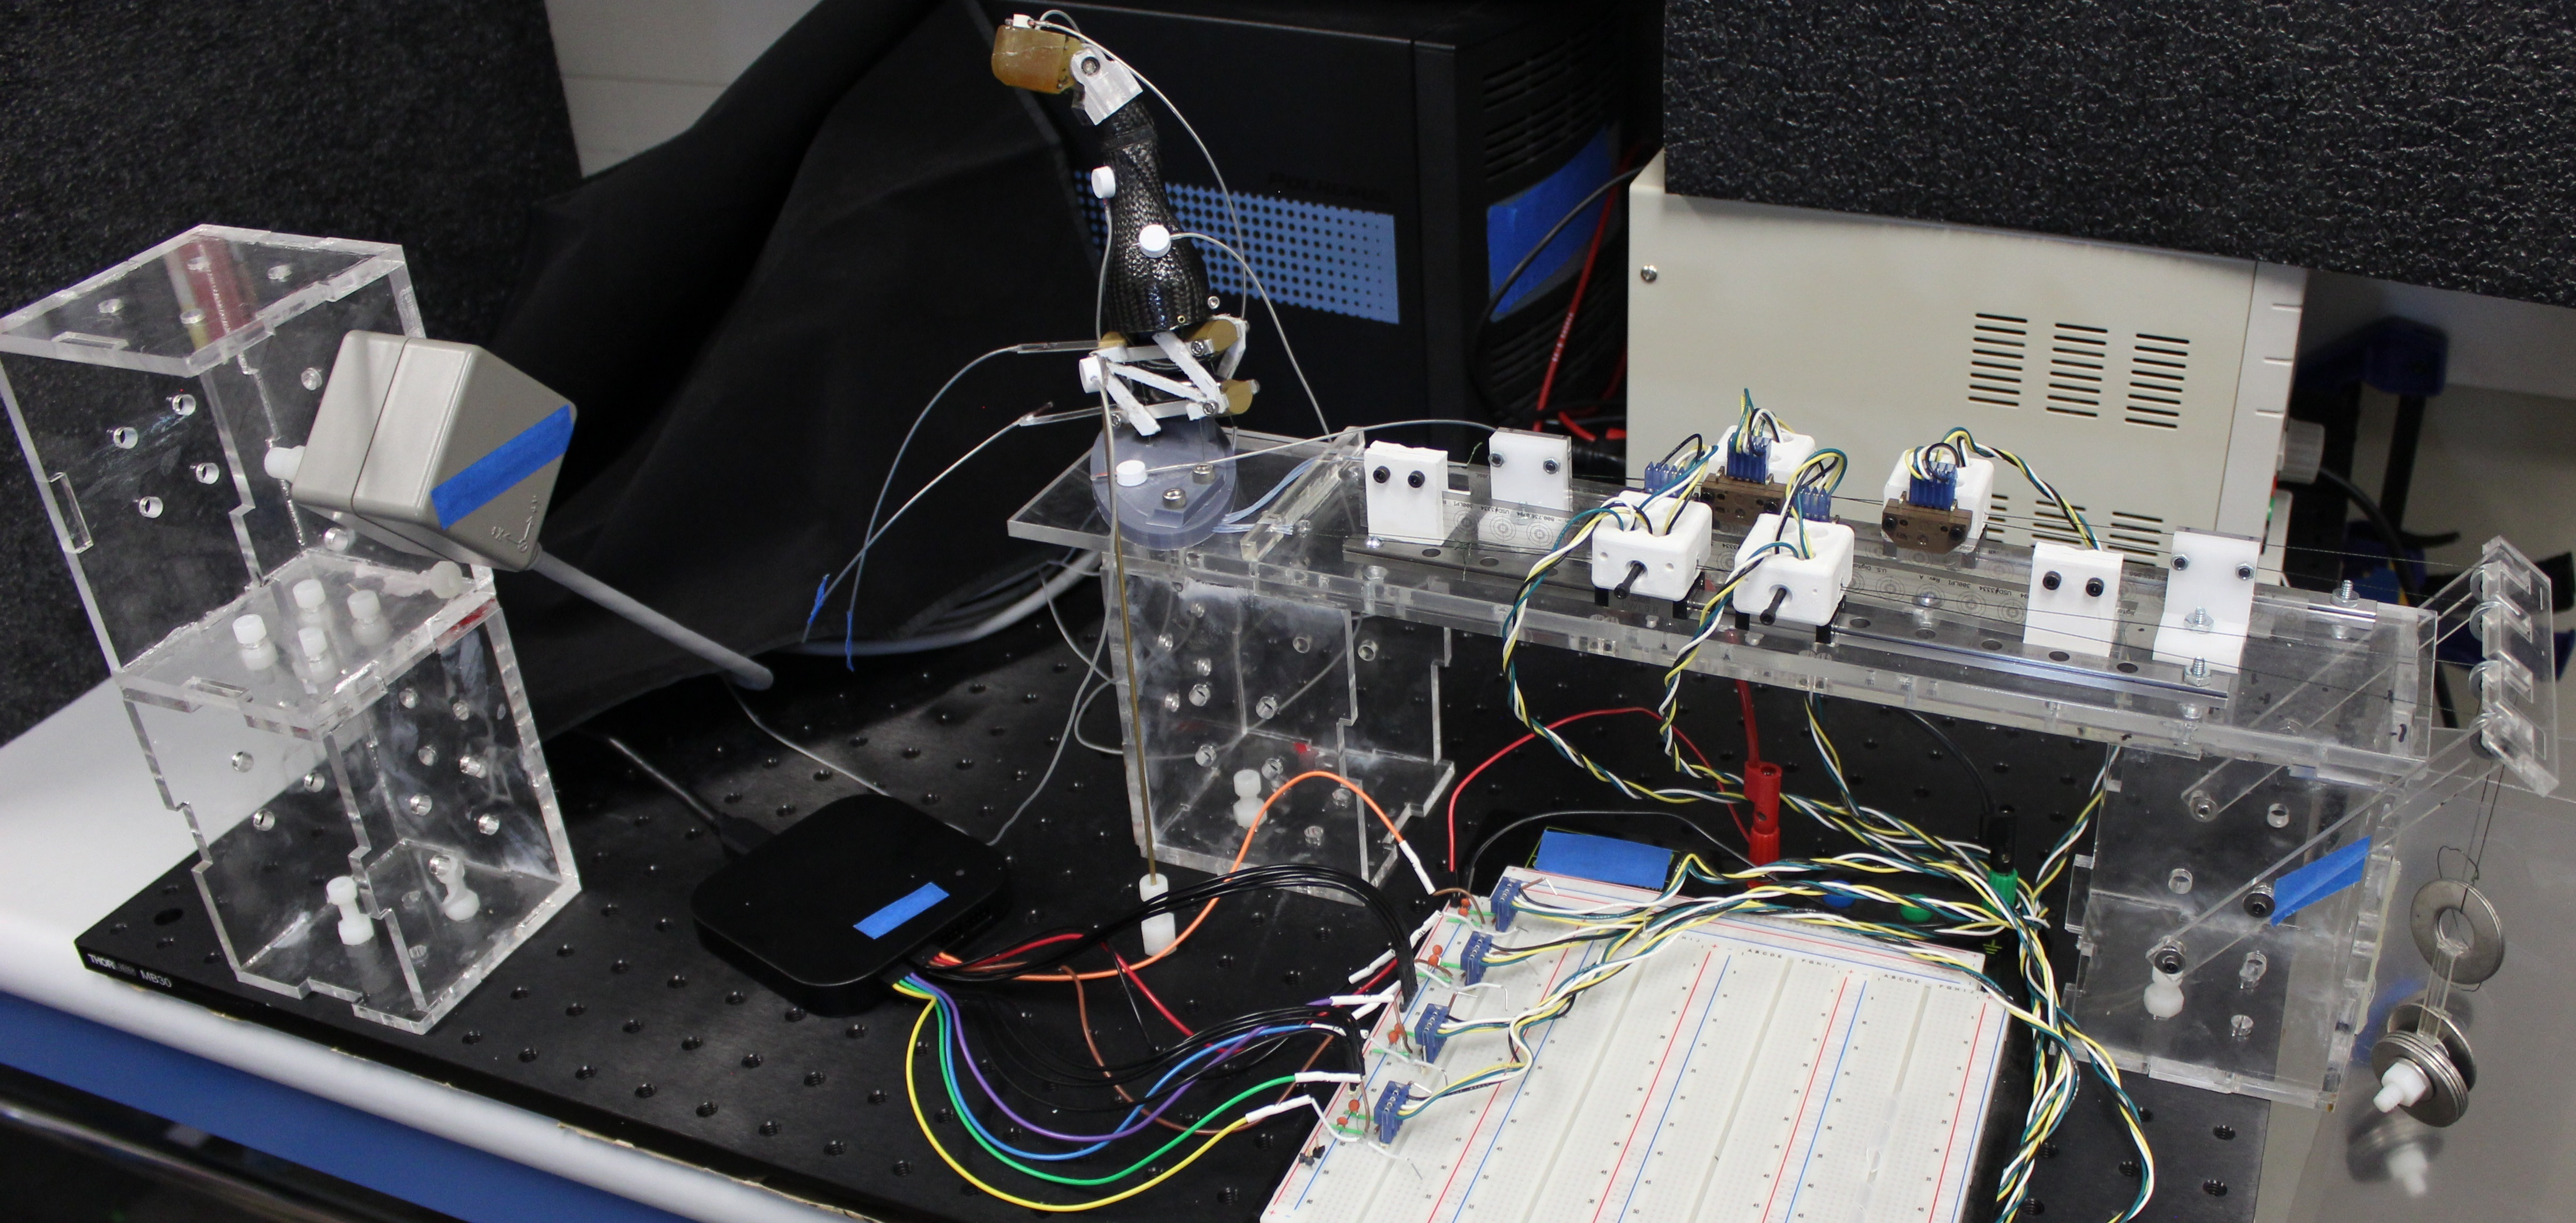
\includegraphics[width = 1\columnwidth]{Figures/overview2v2.JPG}\label{schem}}\\
    \subfloat{(a)}
    {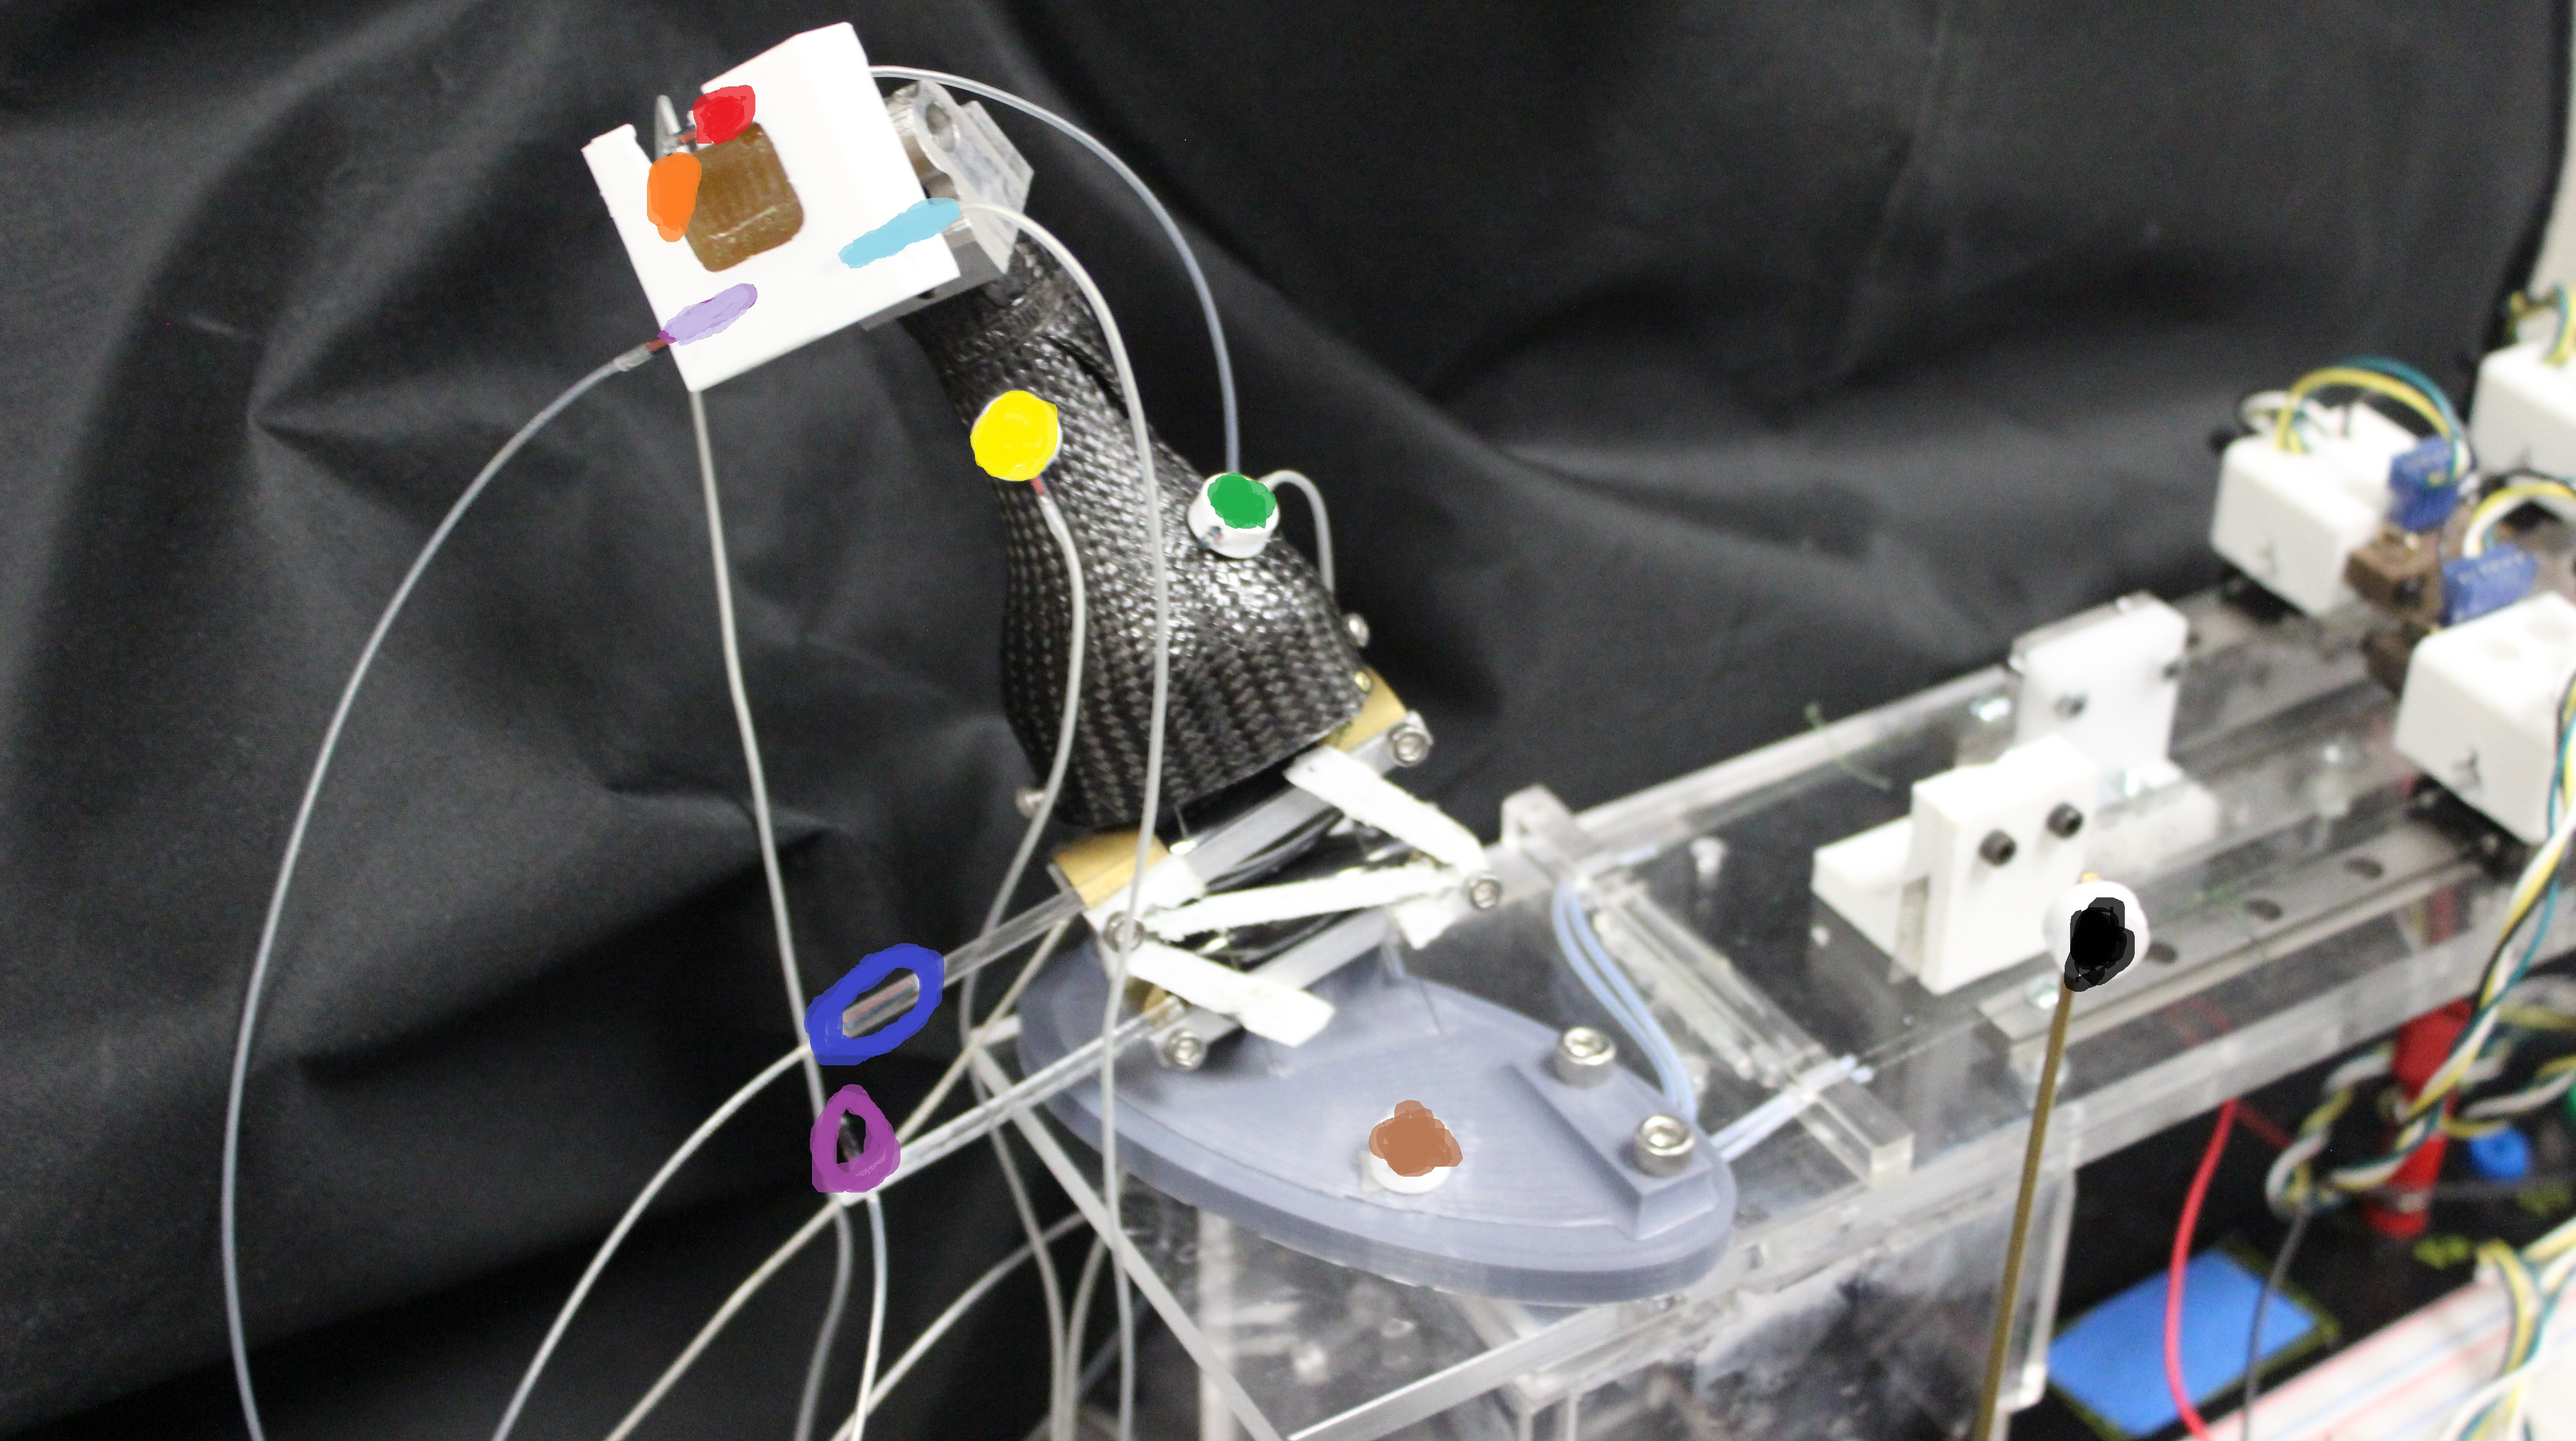
\includegraphics[width = 1\columnwidth]{Figures/D6_v2.JPG}\label{contract}}\\
	\subfloat{(b)}\\
	{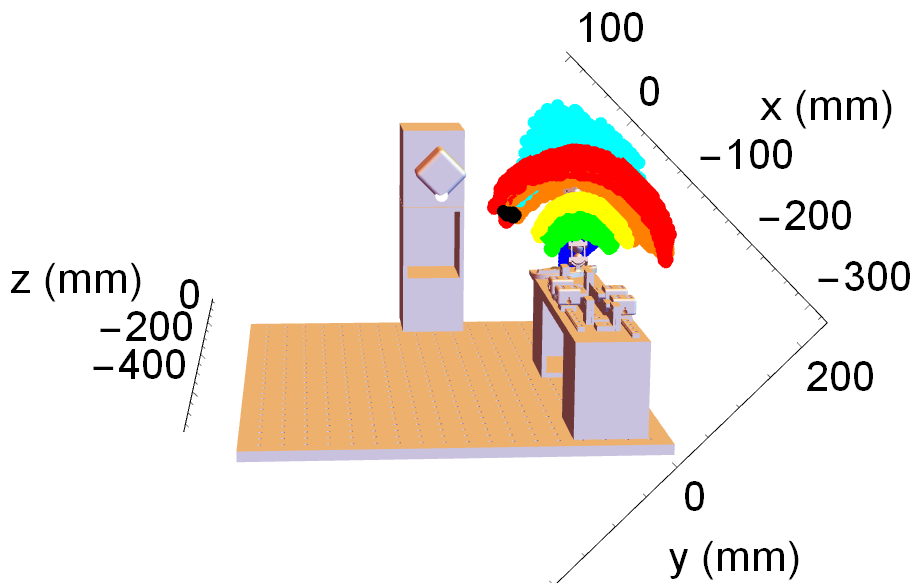
\includegraphics[width = .8\columnwidth]{Figures/F5_v2.PNG}\label{schem2}}\\
	\subfloat{(c)}

	
	\caption{(a) The full experiment is photographed. Data collection is conducted by the Saleae Logic Analyzer and Polhemus Liberty Motion Capture system (at right), and the tendons were kept under a constant tension using weights hung vertically at the termination of each tendon (at left). (b) Data was gathered from the Cartesian positions and Euler-angle orientations of 8 Polhemus Liberty Motion Trackers. (c) the 3D model of our experiment with point cloud data from eight motion trackers, averaged across 20 runs.}\label{workspaces}
\vspace{-6pt}
\end{figure}

\vspace{-6pt}


\begin{figure}
	\centering
	\vspace{7pt}
	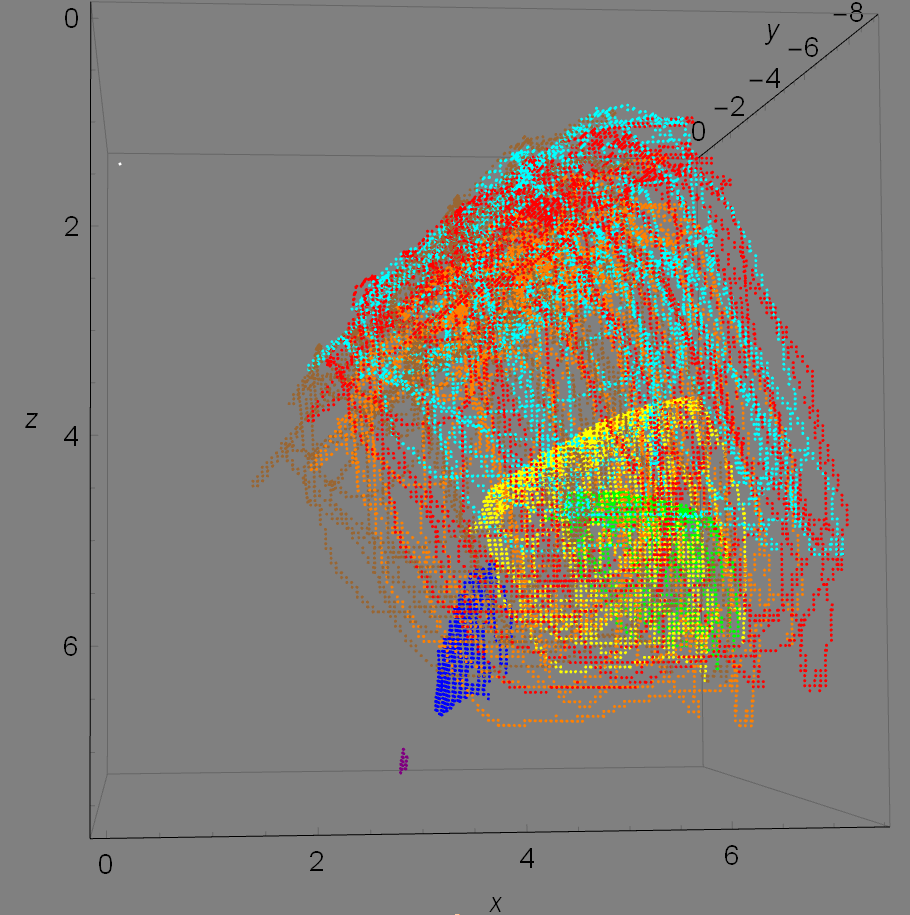
\includegraphics[width = .7\columnwidth]{Figures/H.PNG}\\
	\caption{Example of 1 run of raw sensor data collection from the Polhemus Liberty Motion Tracker. Each run generated around 225K points of data, which over 20 validated runs aggregated close to 4.5 million data points between the tendon excursions and coordinate orientations of the thumb, which itself is raw output from the sensors as a 6-vector (3 positions and 3 angles) at each point. This is reduced to less than 30K points total, by eliminating nearest-neighbors. The discrete colors of the path represent eight points on the phalanges of the thumb assigned to be ``virtual fingers". The end effector is in Cyan and Brown, while the rest of the run's data comes from virtual finger locations. It is inferred that the motion of the CMC is relatively smooth from looking at the lower curves generated by the Polhemus motion trackers secured to the initial links of the thumb.}\label{thumbphoto}
	\vspace{-15pt}

\end{figure}


\section{Prototype Manufacturing}
The novel features to be manufactured are a rolling-ellipsoidal CMC joint with flexure hinges, a hollow carbon-fiber hull on top of single-layer printed PLA with an internal cavity for additional components (sensors, motors, etc.) since there is a continuous fused region in place of the MCP joint. This fused region terminates in a CNC-machined Aluminum 6061 pin joint, which subsequently serves as the thumb's interphalangeal joint (IP) and also mechanically limits the motion of the Distal Phalanx about its axle. The Distal Phalanx's finger pulp constitutes the end effector of the robotic finger.
 
 Starting from the base, the proximal of the two ellipsoids is connected to the palm via geometry realized as a 3D print, made on an Ultimaker 3 Extended out of PLA (MatterHackers, Model M7RDUN0Q). This base is adhered permanently to the bottom of one of the two Rattlesnake Eggs (Amazon, Model B00J1J49E4) which are ceramic and very close to an exact ellipsoid in external geometry. These ellipsoids are aligned about their magnetic poles which enter and exit through one of their minor radii, aligned normal to the thumb itself. This allows for a partial returning force to bring the thumb back into a neutral pose, after it is used.
 
 The CMC's mechanical stops are constituted by machined surfaces which become co-planar during collision, two between each pair of brass Torches, and four on the internal surfaces of the polypropylene flexure hinges. These mechanical stops limit Abduction/Adduction to 55 degrees and Flexion/Extension to 70 degrees, similarly to to those that limit the range of motion of the human hand, and other robotic hands \cite{santos2006reported} \cite{fff}.
 
 The Flexure hinges are machined using a CNC milling machine from 1/8" polypropylene sheets (McMaster, Model 2898K11), and incorporate double C-Type flexure hinges. This is a very well-studied profile for flexure hinges. During manufacturing, the radial parameters of each flexure point were varied and many flexure hinges were produced. A finite element analysis was performed in \textit{ANSYS 18.2}, and predicted that the C-type hinges would behave as modeled and not degrade under the desired range of motion, as Von Mises stresses under the expected range of motion are within the material tolerance of polypropylene. A balance was found in the parameters which allowed the hinge to maintain it's original normal-facing rigidity, and to move through the desired 55 degrees of motion, which is a larger range of motion at this scale than most other flexure hinges in production. The hinges' flexure points are rigidly constrained to lie on the axis of the foci of each ellipse at all times, due to brass ``Torches" which were designed and machined to partially enclose the rattlesnake eggs. The purpose of the Torches is that they are able to rotate about the ellipses' major axis, which allows for the flexion-extension motion (as it is primarily the abduction-adduction motion that deforms the flexure hinges). The brass was similarly machined and produced as the polypropylene. To ensure the CMC joint is held together and the flexure hinges' axes of motion are aligned with their respective foci, small aluminum bars were also installed (McMaster, model 9146T11). Eight 3mm screws were used to secure all components into threaded receiving holes in the brass.
 
 Next, the top rattlesnake egg's reverse side is adhered to another 3D printed geometry, which serves to provide a rigid connection to the carbon fiber. This creates a cavity for other possible components within a single-wall 3D print that is used to lay-up a 2 layer braided carbon fiber bi-axial sleeve (Fibreglast, Model 02609), which is treated with resin to become the outer surface of the robotic thumb. 

\begin{figure}
    \centering
	\vspace{7pt}
	{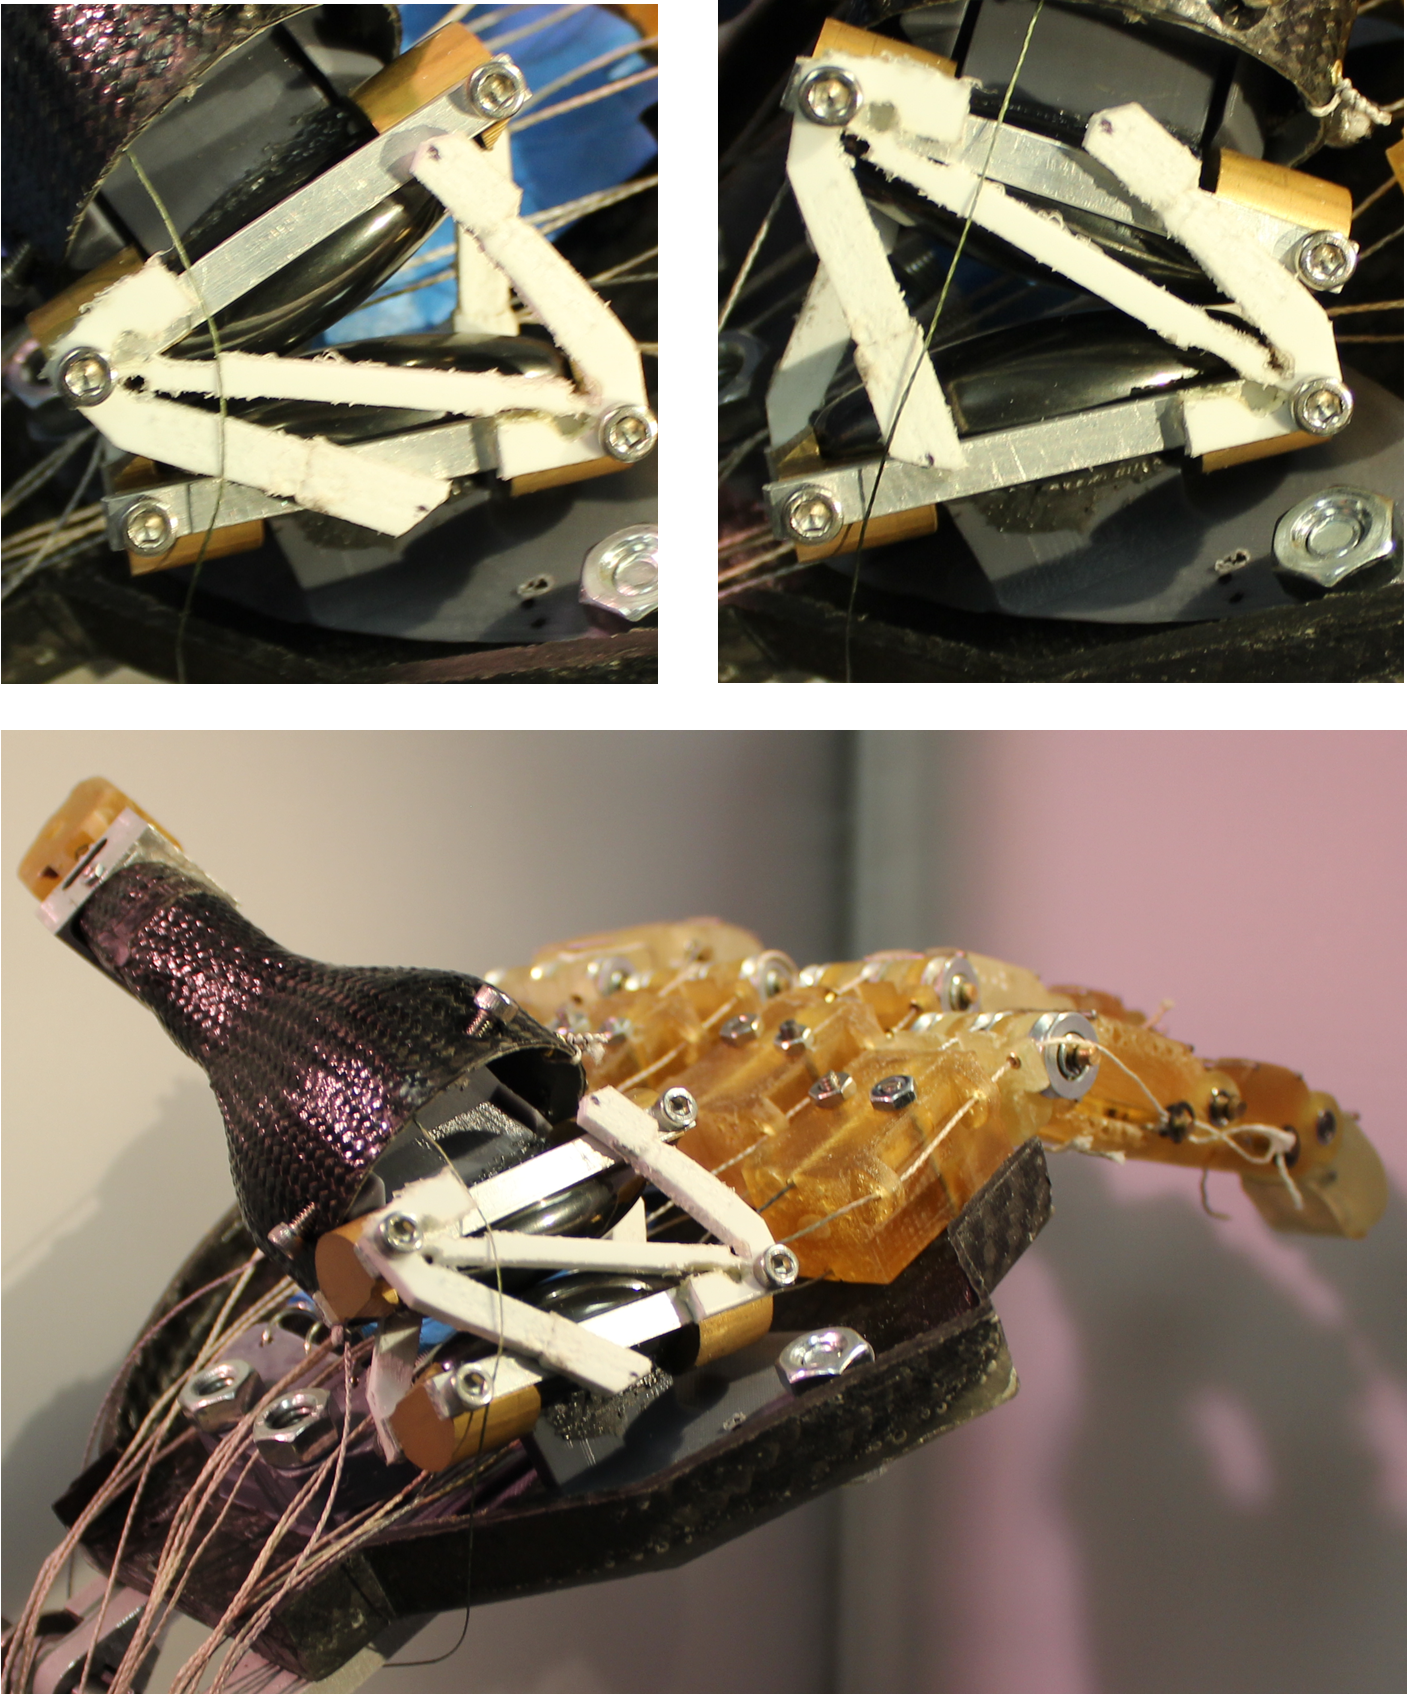
\includegraphics[width = 1\columnwidth]{Figures/garp.png}\label{overload}}\\
	\caption{(Top) The Carpometacarpal Joint of our prototype thumb moving through its range of Adduction-Abduction motion while maintaining maximal Flexion into the palm.
	(Bottom) Our presented thumb prototype installed on the \textit{TU Hand}. }\label{workspaces}
    \vspace{-6pt}
\end{figure}

\section{Data Collection}
Each link's position and orientation is measured via magnetic field distortion-based motion/position sensors running at 240 Hz (Polhemus, Model \textit{Liberty}). Simultaneously, discrete time-step data, which is ultimately re-scaled to 240 Hz intervals for data processing, is measured from the thumb tendon excursion via four 5V Linear Optical Encoders on 300DPI optical rails (USDigital, Model 30035N), read by a Saleae Logic Analyzer (Saleae, Model 0160) and synchronized with the motion sensor data.

The tendons are actuated externally so they cannot slacken at any point in the thumb end effector's workspace. Approximately 500g is vertically loaded at the end of each of the tendons, after they each tie-in to one of four 3D printed blocks on horizontal linear rails, enabling data collection from our linear encoders as shown in Figure 4(a). For each run, this data is compiled as the time-series response of tendon excursion associated with each end effector position throughout the workspace, shown in Figure 5. 

\section{Tracing a relationship between Tendon displacement and End Effector Position}

 The experimental procedure began with fixing the thumb on a stand and placing the tendons under constant tension. The thumb was moved manually over the course of 20 runs, each approximately one minute long, with the purpose of observing the tendon excursions as the thumb is moved throughout its workspace to evaluate the tendon/motion relationship. This is similar to the methodology used in previous work on other robotic fingers \cite{aaah}. Runs continued until the tip of the thumb had traced out a dense set of points throughout its entire workspace. Simultaneously, each link's position in space and orientation at each instant is recorded using the Polhemus motion sensors, while also recording the tendon excursions from their lengths at the starting pose using the Saleae logic adapter. In this way, a point cloud is produced in task space which has tendon excursions and link orientations associated with each one.

To calibrate the end effector, As shown in Figure 4, one must register the center of the Polhemus marker and its orientation to the phalanx geometry (i.e. its location with respect to the CAD model of the part). To do this, the flat side of the DP is pressed into a calibrating fixture outfitted with Polhemus sensors pressed into distinct features already registered to the fixture. The end effector is located on the Distal phalanx in the middle of the thumb ``pulp". This calibrating fixture was 3D printed, to allow for sensing of the end effector without permanently adhering anything to the pulp region of the distal phalanx.

As can be seen in Figure 1, our prototype thumb tendon network was simplified, it only has 4 tendons: one for adduction, abduction, flexion, and extension. Having four tendons arranged in this symmetric way allows for straightforward control design and calibration. The choice was made to use a mechanical tendon and pulley system, instead of localized actuators. This further minimizes the complexity of the device by having as few actuators as possible. Not only does that improve the durability and weight, but it also reduces cost, is more biologically inspired in that it is tendon driven than motors controlling each joint locally, and makes the hand lighter and less bulky, which is important if it is to be used in common tasks.


\begin{figure}
	\centering
	    \vspace{6pt}
	{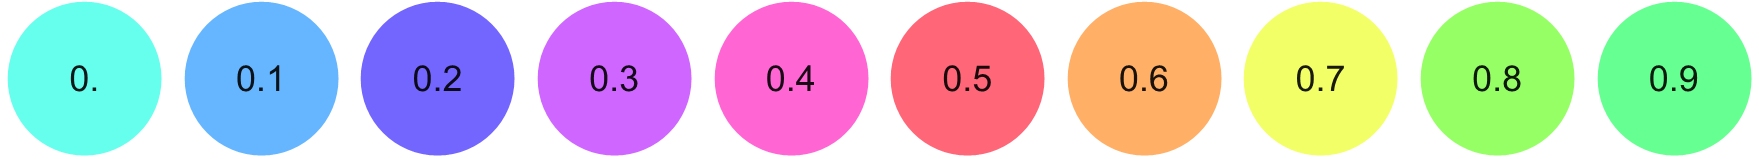
\includegraphics[width = 1\columnwidth]{Figures/E20.PNG}\label{schem}}\\
		\subfloat{Normalized SMM Scale}
	{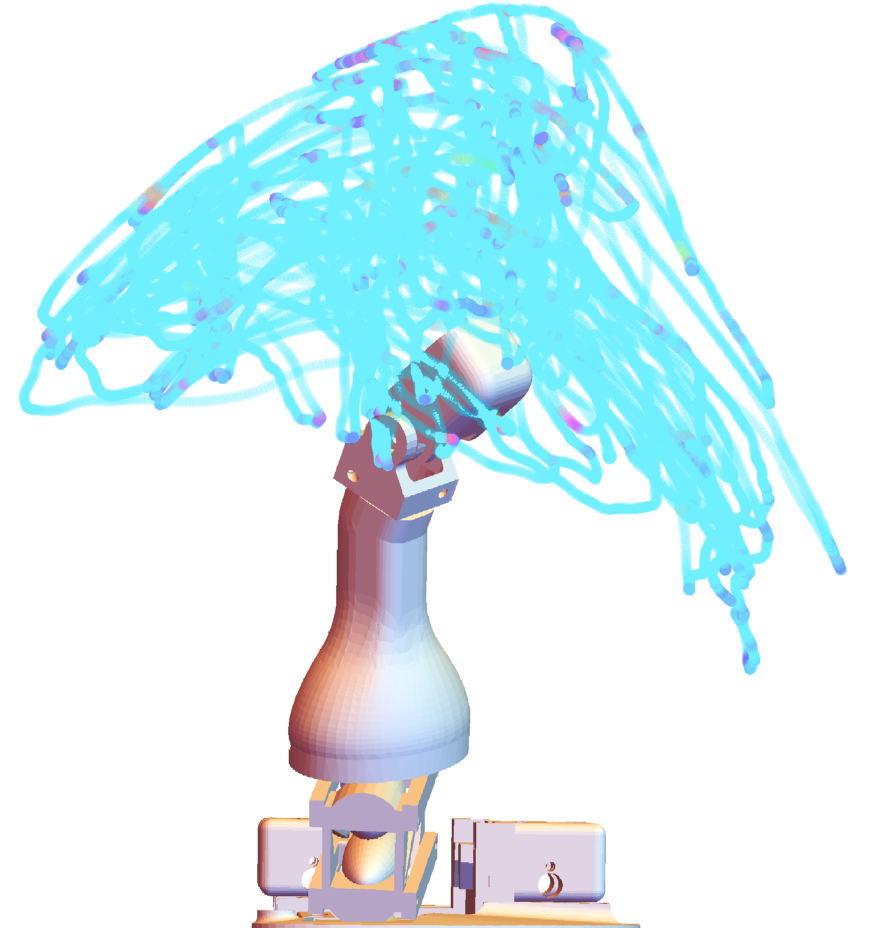
\includegraphics[width = 0.8\columnwidth]{Figures/E21.PNG}\label{contract}}\\
	\subfloat{(a)} \\
	{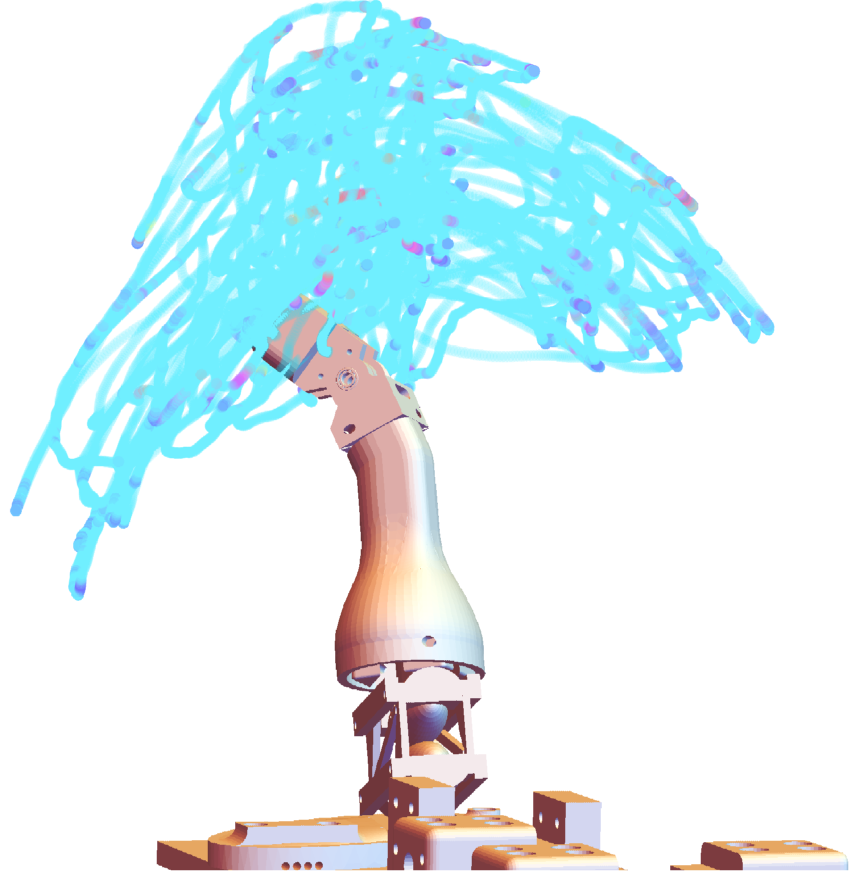
\includegraphics[width = 0.5\columnwidth]{Figures/E2.PNG}\label{overload}}{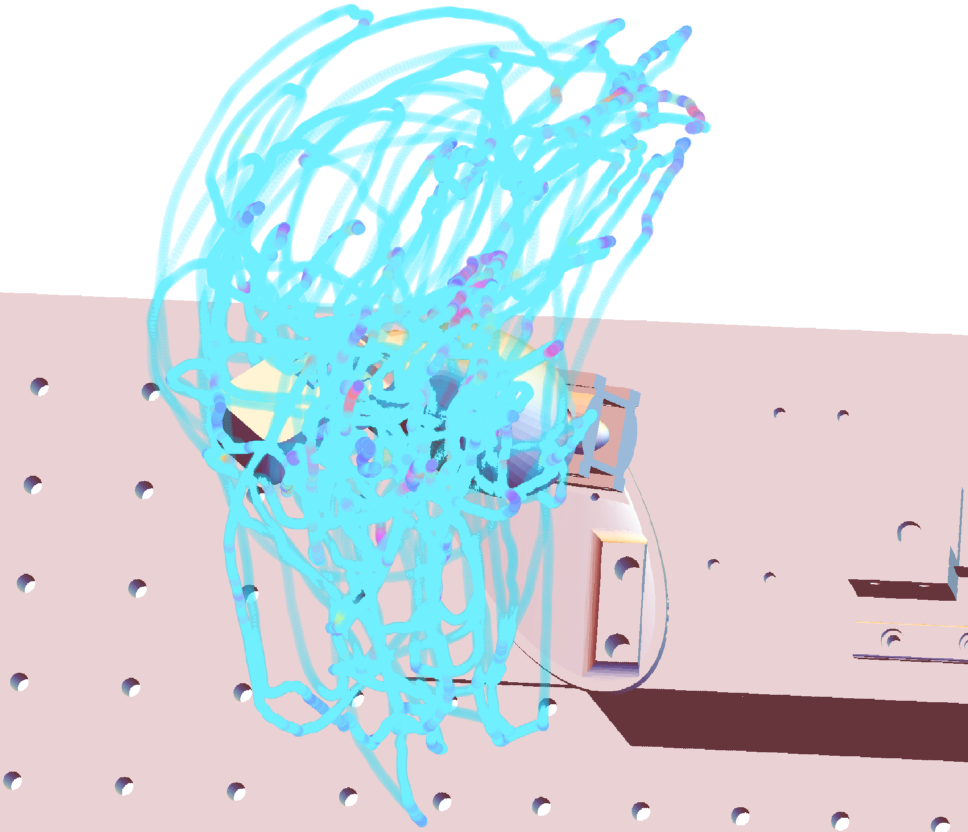
\includegraphics[width = 0.5\columnwidth]{Figures/E4.PNG}\label{overload}}\\
	\subfloat{(b)} \hspace{3cm}  \subfloat{(c)} \\
	\caption{The view of the relative velocity mapping across the excursion of the end effector through it's workspace, viewed from the perspective of (a) the palm, (b) the wrist, (c) collinear with the axis of the metacarpal linkage, and (d) behind the palm of the hand. The calculated value of the SMM at each point is represented by that point's color saturation as indicated above.
	}\label{workspaces}
%\vspace{-7pt}
\end{figure}



\section{The Simplified Manipulability Metric: Quantifying the Smoothness of mapping between tendon excursion velocity and End Effector Velocity.}

\begin{equation}
A=\sqrt{{\frac{\Delta l1}{dt}}^{2}+{\frac{\Delta l2}{dt}}^{2}+{\frac{\Delta l3}{dt}}^{2}+{\frac{\Delta l4}{dt}}^{2}}
\end{equation}

\begin{equation}
B=\sqrt{{\frac{\Delta x}{dt}}^{2}+{\frac{\Delta y}{dt}}^{2}+{\frac{\Delta z}{dt}}^{2}}
\end{equation}

\begin{equation}
w=\frac{B}{A}
\vspace{10pt}
\end{equation}

To assess the function of the experimental thumb in it's current state, a metric called the Simplified Manipulability Metric (SMM) is adapted from a recently introduced metric to evaluate the KITECH Hand, known as the Manipulability Metric (MM) \cite{kitech}. Equation 3 represents a scalar quantity describing the variance of the tendon movement velocity relative to the end effector movement velocity through it's workspace in time, as represented in Cartesian coordinates. With it, we can deduce what region of the workspace might be the best operating region within the workspace, because the four tendon displacements in Equation 1 ($\Delta l1-\Delta l4$) do not appear to fluctuate wildly for small workspace displacements, and vice versa. This is essentially a simplified form of finding the numerical Jacobian between the tendon excursions and the end effector positions, except instead of searching locally in all possible directions within the full data set, it is only computed backwards and forwards along the path taken as the data was collected. Estimating the full Jacobian is much more numerically intensive and is not expected to be significantly increase accuracy. This metric represents how well-conditioned the mapping is between the controlled tendon output position and the observed end effector trajectory. This metric was used to create all the graphics seen in Figure 7. Values of the normalized SMM close to unity imply the relative velocities are further apart than usual, while values close to zero imply the relative velocities at that point are similar in magnitude.

It is possible some of the increases in relative velocity are due to ``catch points" on the CMC, where the tendons pass freely over the ellipsoids, but may intersect briefly with metal surfaces. This issue could be avoided by routing all tendons more distally to the ellipsoids, and measuring their dexterity by considering the device as a tendon actuated parallel mechanism \cite{dex}. The Simplified Manipulability Metric (SMM) is used to quantify the ability of the thumb to manipulate objects at each path point. 

%Equations were here in first submitted draft 

The SMM is similar in spirit to the MM, but should be significantly faster to compute when processing experimental or real-time data. It can be shown from the equations derived in their previous work that our SMM is a re-scaled equivalent to the Manipulability Metric. The MM is supposed to describe the volume of the Manipulability Ellipsoid, and thus represents the functionality of the hand \cite{kitech}. The SMM is computed from the experimental data gathered in Section VI, and looking at Figure 7, the SMM does not deviate significantly from zero, indicating little change in the relative velocities of the tendons and end effector paths; this indicates our prototype is manipulable almost anywhere in its workspace. Figure 7 also shows the higher values of the metric occurs on the edge of the point cloud; this is likely due to nonlinearities introduced into the end effector's path from the collision of the CMC's mechanical stops, or due to specific thumb pose sequences that cause tendons to catch on other features and deviate from their normal path. 

\section{Conclusion}
A robotic thumb design is proposed which attempts to embed the stability, precision, and robustness of the human thumb into a simplified, inexpensive design. This design uniquely captures the range of motion of the CMC while preserving the size of the thumb's workspace, even with the MCP joint fixated as in an Arthrodesis patient. It utilizes fewer joints than a human thumb, and utilizes flexure hinges so that the joint constraints are well-conditioned, improving upon our previous work. At the base of the thumb, a Rolling-Ellipsoidal Joint with two degrees of freedom is constrained to rolling without slipping by counter-balancing Flexure Hinges. This joint is inspired by the Carpometacarpal Joint of the Human Thumb, which has proven difficult to design, build and control for traditional robotics in a functional way. The complex geometry between the equivalent halves of the joint is realized using inexpensive ceramic magnets, which approximate ellipsoidal hemispheres normal to their magnetic poles. The smoothness of this relationship is quantified using the normalized relative velocity of the tendon and end effector space vectors, and this quantity mapped across the workspace to show visually where the motion of the end effector can not be as precisely controlled by setting tendon excursions. Efforts are underway to implement the robotic thumb design into robotic hands, starting with the underactuated, biomimetic TU Hand \cite{das}. Future work can also use this data to isolate irregular areas of the workspace, and have already helped identify and resolve issues in the tendon routing about the rolling ellipsoidal CMC design. A similar, but more descriptive measure would be the Jacobian from the tendon excursions to the joint angles, and this will also be a part of future work.


\begin{thebibliography}{99}

%1
\bibitem{vfingers}Cutkosky, Mark R. ``On grasp choice, grasp models, and the design of hands for manufacturing tasks." IEEE Transactions on robotics and automation 5, no. 3, 269-279,  1989.
%2
\bibitem{ss}Kormushev, Petar, Sylvain Calinon, Ryo Saegusa, and Giorgio Metta. ``Learning the skill of archery by a humanoid robot iCub." In 2010 10th IEEE-RAS International Conference on Humanoid Robots, pp. 417-423. IEEE, 2010.
%3
\bibitem{santos2006reported} Santos, Veronica J., and Francisco J. Valero-Cuevas. ``Reported anatomical variability naturally leads to multimodal distributions of Denavit-Hartenberg parameters for the human thumb." IEEE Transactions on Biomedical Engineering 53, no. 2, 155-163, 2006.
%4
\bibitem{niehues} Niehues, Taylor D., and Ashish D. Deshpande. ``Variable thumb moment arm modeling and thumb-tip force production of a human-like robotic hand." Journal of biomechanical engineering 139, no. 10,  101005, 2017.
%5
\bibitem{nana} Nanayakkara, Visakha K., Giuseppe Cotugno, Nikolaos Vitzilaios, Demetrios Venetsanos, Thrishantha Nanayakkara, and M. Necip Sahinkaya. ``The role of morphology of the thumb in anthropomorphic grasping: a review." Frontiers in Mechanical Engineering 3, 5, 2017.
%6
\bibitem{steiger}Steiger, R., and G. Segmüller. ``Arthrodesis of the metacarpophalangeal joint of the thumb. Indications, technic, arthrodesis angle and functional effect." Handchirurgie, Mikrochirurgie, plastische Chirurgie: Organ der Deutschsprachigen Arbeitsgemeinschaft fur Handchirurgie: Organ der Deutschsprachigen Arbeitsgemeinschaft fur Mikrochirurgie der Peripheren Nerven und Gefasse: Organ der V... 21, no. 1, 18-22, 1989.
%7
\bibitem{biorob}Pulleyking, Spenser, Dipayan Das, and Joshua Schultz. ``Simplified robotic thumb inspired by surgical intervention." In 2016 6th IEEE International Conference on Biomedical Robotics and Biomechatronics (BioRob), pp. 1200-1206. IEEE, 2016.

%8
\bibitem{iCub}Schmitz, Alexander, Ugo Pattacini, Francesco Nori, Lorenzo Natale, Giorgio Metta, and Giulio Sandini. ``Design, realization and sensorization of the dexterous iCub hand." In 2010 10th IEEE-RAS International Conference on Humanoid Robots, pp. 186-191. IEEE, 2010.
%9
\bibitem{pisahand}Gao, Geng, Anany Dwivedi, Nathan Elangovan, Yige Cao, Lucy Young, and Minas Liarokapis. ``The New Dexterity adaptive, humanlike robot hand." In IEEE International Conference on Robotics and Automation. ICRA, 2019.
%10
\bibitem{kingcakebaby}Cui, Lei, Cupcic, Ugo, Dai, Jian.  An Optimization Approach to Teleoperation of the Thumb of a Humanoid Robot Hand: Kinematic Mapping and Calibration. ASME Journal of Mechanical Design. 136. 091005-091005, 2014.

%\bibitem{pisahand}Schectman, Leonard A. ``Artificial robotic hand." U.S. Patent 5,080,682, issued January 14, 1992.

%11
\bibitem{havd}Odhner, Lael U., Leif P. Jentoft, Mark R. Claffee, Nicholas Corson, Yaroslav Tenzer, Raymond R. Ma, Martin Buehler, Robert Kohout, Robert D. Howe, and Aaron M. Dollar. ``A compliant, underactuated hand for robust manipulation." The International Journal of Robotics Research 33, no. 5, 736-752, 2016.

%12
\bibitem{yodel}Schotborgh, Wouter O., Frans GM Kokkeler, Hans Tragter, and Fred JAM van Houten. ``Dimensionless design graphs for flexure elements and a comparison between three flexure elements." Precision Engineering 29, no. 1, 41-47, 2005.

 %13
\bibitem{homies}Das, Dipayan, Nathanael J. Rake, and Joshua A. Schultz. ``Compliantly underactuated hands based on multiport networks." 2016 IEEE-RAS 16th International Conference on Humanoid Robots (Humanoids). IEEE, 2016.

%14
\bibitem{fff}Wang, Hairong, Shaowei Fan, and Hong Liu. ``Thumb configuration and performance evaluation for dexterous robotic hand design." Journal of Mechanical Design 139, no. 1,012304, 2017.

%15
\bibitem{aaah}Rake, Nathanael J., Spencer P. Skinner, Gavin D. O'Mahony, and Joshua A. Schultz. ``Modeling and implementation of a simplified human tendon structure in a robotic finger." In 2016 6th IEEE International Conference on Biomedical Robotics and Biomechatronics (BioRob), pp. 120-125. IEEE, 2016.

%16
\bibitem{kitech}Lee, Dong-Hyuk, Jae-Han Park, Sung-Woo Park, Moon-Hong Baeg, and Ji-Hun Bae. ``KITECH-hand: A highly dexterous and modularized robotic hand." IEEE/ASME Transactions on Mechatronics 22, no. 2, 876-887, 2016.

%17
\bibitem{dex}Kurtz, Ronald, and Vincent Hayward. ``Dexterity measure for tendon actuated parallel mechanisms." In IEEE Intl. Conf. on Advanced Robotics, pp. 1141-1146. 1991.


%18
\bibitem{das}Das, Dipayan, Nathanael J. Rake, and Joshua A. Schultz. ``The TU Hand: Using Compliant Connections to Modulate Grasping Behavior." In Robotic Grasping and Manipulation Challenge, pp. 57-83. Springer, Cham, 2016.

\end{thebibliography}


\end{document}
